\chapter{Introduction}\label{introduction}

\section{Background and Motivation}

The CESAR project aim to use low cost sensor kit to prototype applications using physiological signals related to heart rate, brain activity, oxygen level in blood to monitor sleep and breathing related illnesses, like Obstructive Sleep Apnea (OSA). Side effects of OSA do not only cause sleepiness during day time (which might affect daily chores), but also serious illnesses like diabetes and cardiac dysfunctions. Statistically speaking, it is estimated that about 25\% of the adult population in Norway has OSA, but only 10\% of them are diagnosed. A major problem with diagnosing OSA is polysomnography in \textit{sleep laboratories} \cite{cesar}. This is both really expensive and inefficient due to lacking capacity to perform sufficient tests with patients. Hence, the CESAR project aims to contribute to this situation with a low-cost Android and BiTalino based system to tackle these problems in a minimal invasive approach. 

The project has been developed by various people over the years, and the system has been divided into three parts (illustrated in Figure \ref{fig:parts}). The data acquisition part, the data streams dispatching part, and the application part. The first two parts are already implemented (summarized in the section below), thus, the last part is what we will be focusing throughout this thesis. 

\begin{figure}
    \centering
    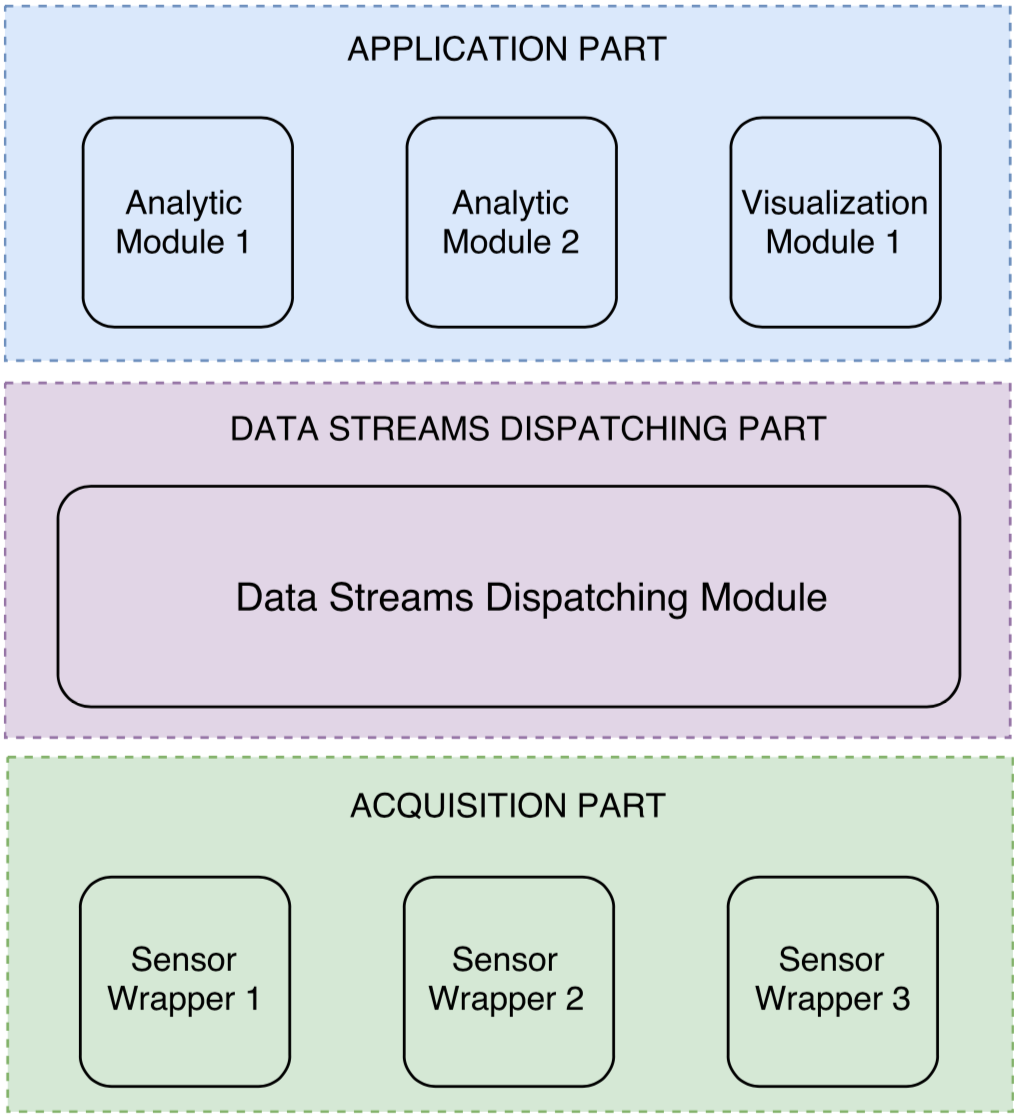
\includegraphics[width=0.5\textwidth]{images/parts.png}
    \caption{Structure of the project, separating functionality into three independent layers \cite{daniel}}
    \label{fig:parts}
\end{figure}

\section{Problem Statement}

The market has new and affordable sensors that can aid with the data acquisition, which we seamlessly can integrate with the extensible data streams dispatching tool. The Flow sensor is an interesting sensor source due to its versatility and adaptability of collecting breathing data and connecting to devices with the BlueTooth protocol. 

As for the state of this thesis: (i) applications which supports the Flow sensor has not been designed for end-users, in essence, they provide no user-friendly interface that allows for sharing of the data. In order to extract the data from these applications, the mobile device has to be connected with a PC over USB for data transfer; (ii) there is no sensor wrappers that support the Flow sensor with the data streams dispatching tool in the CESAR project; and (iii) the data streams dispatching tool is not ready to be used by the end-users, because the project facilitates no user-friendly interface for users to record the data from the supported sensor sources.

As such, we look into designing and implementing an Android application (Nidra) that record, share, and analyze breathing data over an extended period (e.g., during sleep) by using the Flow sensor. Additionally, we want to facilitate an extensible application such that future developers can extend functionality or enrich the data in Nidra. In the end, we can hopefully strengthen the analysis of abnormal sleeping patterns to decreasing the risk of the symptoms they may come as a consequence. Also, as a bi-product, the application can be used in other fields of studies (e.g., physical activities). As the scope of this thesis, we focus on the completion of three main goals:

\begin{description}
    \item[Goal 1] Integrate the support for Flow sensor by creating a sensor wrapper that connects with the extensible data streams dispatching tool.
    \item[Goal 2] Research and develop a user-friendly application which facilitates collection of breathing data with the Flow sensor, sharing of the data, and analysis of the data with the use of the extensible data streams dispatching tool.
    \item[Goal 3] Create an extensible solution such that the developers can create standalone applications that integrate with Nidra. 
\end{description}

As part of the goals of this thesis, we also define three system requirements to keep in mind while designing and implementing the application. The three system requirements are the following: 

\begin{description}
    \item[Requirement 1] The application must provide an interface for the patient to (i) record physiological signals (e.g., breathing data); (ii) present the results; and (iii) share the results.
    \item[Requirement 2] The application must ensure that upon sensor disconnections, the connectivity is reinstated to minimize the data loss and its effects on the data analysis.
    \item[Requirement 3] The application must provide an interface for the developers to create modules that integrate with the application.
\end{description}



\section{Limitations}
Based on the goals and requirements stated in previous section, the scope of this thesis is to design and implement an application capable of recording breathing data obtained by the Flow sensor kit over an extended period. 

We limite the scope to integrating the support for the Flow sensor kit in Nidra, and exluded to test for already integrated sensor sources (e.g., Bitalino). Further, with the Flow sensor kit provided under development, we restricted the design to collect respiration (breathing) data (opposed to hearth-rate or other physiological data).

The application is designed to collect breathing data; we do not perform any analysis to predict or detect sleeping disorders based on the data. However, we facilitate for future developers to utilize the data provided by Nidra to perform such task.

Finally, the implementation is Android specific as the previous work performed on the project is designed soley for Android applications. 

\section{Research Method}
The work in this thesis can be classified as \textit{computing research} with a principle approach of an \textit{engineering method} as described in \cite{Glass_1995}. The engineering method (evolutionary paradigm) is to: (i) observe existing methods, (ii) propose a better solution, (iii)  build or develop artifacts\footnote{human-manufactured objects produced during the development}, and (iv) measure and analyze until no further improvements are possible. The report identifies patterns amongst various principle approaches and categorizes the the patterns into phases: \textit{(i) informational phase}, \textit{(ii) propositional phase}, \textit{(iii) analytical phase}, and \textit{(iv) evaluation phase}. Below, we give a brief description of each phase and discuss how our work fits into each of them. 

\subsection{Informational Phase}
The informational phase according to the report is to \textit{"gather or aggregate information via reflection, literature survey, people/organization survey, or poll"}

In this thesis, we survey previous related work in the field of detecting, analyzing, and diagnosing sleep related-breathing disorders on a mobile device. A vast amount of the work, use various techniques and methods to improve the diagnosis of the disorders (e.g., using the microphone and the accelerometer in the mobile device). However, the applications are scattered around in the real-world, resulting in the patients have operate with multiple applications that are intended to do the same thing. Our intention is to create an generalized application, that reduce the development time for developers/researchers, and for patients to operate with one application for diagnosis and examination of sleep apnea. As such, we allow future developers expedite innovation in the research and study of sleep-related breathing disorders, as well as allowing patients to operate with one application. 

\subsection{Propositional Phase}
The propositional phase according to the report is to \textit{"propose and/or formulate a hypothesis, method or algorithm, model, theory, or solution"}

The solution proposition in this thesis is to create an application which will be used to record, share, and analyze breathing data collected over an extended period. We want to extend the CESAR project by providing an user-interface to the patient to perform these tasks while using the tools that the project facilitates. Mainly, we want to use the data streams dispatching tool in order to manage current and future sensor sources. In which, we proceed to add support for the Flow sensor kit. In the end, we wish to facilitate an application that is used by the patients to record their breathing data during sleep and to share the data between researchers/doctors. As such, we aid in analyzing the data to detect sleep-related breathing disorders (e.g., obstructive sleep apnea) from home. 

\subsection{Analytical Phase}
The analytical phase according to the report is to \textit{"analyze and explore a proposition, leading to a demonstration and/or formulation of a principle or theory"}

With the proposition of this thesis, we analyze the tasks and separate them into concerns. Each concern has design choices that combined fulfills the goals of this thesis. As a demonstration, we realize the design choices by implementing them as an Android application, called Nidra. 

\subsection{Evaluation Phase}
The evaluation phase according to the report is to \textit{"evaluate a proposition or analytic finding by means of experimentation (controlled) or observation (uncontrolled, such as a case study or protocol analysis), perhaps leading to a substantiated model, principle, or theory"}

Based on the requirements and goal of this thesis, we evaluate the application by conducting experiments. Some of the experiments include participants that perform various tasks, such that we can observe the outcome of the tasks on participants without prior knowledge or experience of the application. In the end, we evaluate and conclude whether the goals and requirements of this thesis are sufficient.

\section{Contributions}
Over the course of this thesis, we designed and implemented an application for collecting, sharing, and analyzing breathing data, called Nidra. Also, we provided an extensible solution for developers to create modules that enrich the data and the functionality of Nidra. The motivation of application is to aid in collecting breathing data with the Flow sensor kit over an extended period. The patient should be able to send the records with breathing data to researchers/doctors, in which they can analyze and diagnose the patient for sleep apnea. However, the application can also be used in other fields of study (e.g., physical activity)  due to its extensible approach of design. As defined in our problem statement, we set three research goals with three system requirements. Below, we present the goals and requirements and describe how our system meets them:

\begin{description}
    \item[Requirement 1] \textit{The application should provide an interface for the patient to 1) record physiological signals (e.g., during sleep); 2) present the results; and 3) share the results.}
    
    In the design of this thesis, we separate the tasks into concerns. Respectively, the task to record breathing data is part of the \textit{recording} concern, where we discuss the possibilities of realizing this functionality. Likewise, we separate the functionality to present the results in \textit{analysis} concern, and to share the result in \textit{sharing} concern. Moreover, we implement the concerns in Android and evaluate whether the functionalities are sufficient. Based on the results, we conclude that the requirements are fulfilled to its extent.
    
    \item[Requirement 2] \textit{The application should ensure a seamless and continuous data stream, uninterrupted from sensor disconnections and human disruptions.}
        
    As part of the recording concern, we discuss various methods of implementing the functionality of having a continuous data stream. The solution is to reconnect with the sensor when we detect that the application is not receiving samples within a time frame. The proposition of design was implemented and evaluated in the experiments, and the functionality works as intended.

    \item[Requirement 3] \textit{The application should provide an interface for the developers to create modules to enrich the data from records or extend the functionality of the application.}

    In the concern for \textit{modules}, we design the functionality of having separate applications that leverage the data provided by Nidra. The design is that Nidra provides a module with records on module-application launch. As such, the developers can create independent applications without having to understand how Nidra operates. The functionality was tested in the evaluation and worked seamlessly.

\end{description}

With the requirements fulfilled, we can look at how Nidra solves our three research goals.

\begin{description}
    \item[Goal 1] \textit{Integrate the support for Flow sensor kit with the extensible data streams dispatching tool.}
    
    In the implementation of this thesis, we added the support for the Flow sensor kit in the data streams dispatching module. We created a separate application that solely connects with the sensor sources which uses BlueTooth LowEnergy protocols to communicate.

    \item[Goal 2] \textit{Research and develop a user-friendly application which facilitates collection of breathing data with the use of the extensible data streams dispatching tool.}
    
    With the system requirements, we fulfilled this goal in the design and implementation of this thesis. The application is precautious to the environment (e.g., the application is most likely to be used during the night) of use. Also, we ensured to limit the action a user can perform on each screen. As such, we created an efficient but straightforward application that can collect breathing data over an extended period using the data streams dispatching tool. 
    
    \item[Goal 3] \textit{Create an extensible solution such that the developers can integrate stand-alone applications in our application.}

    As part of the system requirement, we designed the application to support the integration of standalone-applications, called modules. These modules utilize the data forwarded by Nidra on launch. The developers of the modules do not need to know how the Nidra operates and can create functionality extends the functionality of Nidra (e.g., a module predict sleep apnea with machine learning) or enrich the data (e.g., with other physiological data).   
\end{description}



\section{Thesis Outline}
The thesis is divided into three parts, which the following list presents a general overview of:

\begin{itemize}
    \item Part 1: \textbf{Introduction \& Background}
    \begin{description}[font=\normalfont\itshape]
        \item[Chapther 2: Background] presents the background material necessary for understanding the fundamentals in this thesis. It starts by introducing the CESAR project and the tools provided for data acquisition. Then, an overview of the Android operating system architecture and components are 
        \item[Chapther 3: Related Work] presents the related work focusing on creating a mobile applicaton to collect physiological data in order to diagnose sleep apnea. Finally, we discuss why our solution is an improvement to the related work.
    \end{description}

    \item Part 2: \textbf{Design \& Implementation}
    \begin{description}[font=\normalfont\itshape]
        \item[Chapther 4: Analysis and High-Level Design] encompasses the functional requirements, the design purposal, and the structure of the data in the application.
        \item[Chapther 5: Implementation] realizes the design purposal in Android, with the use of the previous work.
    \end{description}

    \item Part 3: \textbf{Evaluation \& Conclusion}
    
    \begin{description}[font=\normalfont\itshape]
        \item[Chapther 6: Evaluation] conducts various experiements in order to tests if the system requirements is fullfilling.
        \item[Chapther 7: Conclusion] discuss the objectives and the overall goal of the thesis, with suggestions to future work.
    \end{description}

\end{itemize}

